\chapter{Introduzione}

\section{Calcolo parallelo}

Il calcolo parallelo è un paradigma di programmazione che consente di eseguire più operazioni contemporaneamente, sfruttando la potenza di elaborazione di più unità di calcolo. A differenza dello pseudoparallelismo, che simula l'esecuzione simultanea di più processi su un singolo processore, il calcolo parallelo utilizza effettivamente più processori o core per eseguire compiti in parallelo. 

Questo paradigma è utile perché riduce i tempi di esecuzione e aumenta la dimensione dei dati processabili, consentendo di affrontare problemi più complessi e di ottenere risultati più rapidamente. 

\section{Limiti del calcolo parallelo}

\subsection{Caso ideale di parallelizzazione}
Per comprendere i limiti del calcolo parallelo è utile partire da un modello ideale. 
Supponiamo che un programma sia completamente parallelizzabile, cioè che tutto il lavoro possa essere suddiviso tra più unità di calcolo senza alcuna parte sequenziale.

Se $T_0$ indica il tempo di esecuzione del programma in modalità sequenziale e $N$ il numero di unità di calcolo disponibili, il tempo di esecuzione ideale del programma parallelo sarebbe:

\[
T_L(N) = \frac{T_0}{N}
\]

In questo caso il tempo di esecuzione diminuisce linearmente all'aumentare del numero di processori. 
Lo speed-up ottenuto è quindi:

\[
S_L(N) = \frac{T_0}{T_L(N)} = N
\]

Questo significa che, in condizioni ideali, raddoppiare il numero di unità di calcolo dimezza il tempo di esecuzione. 
In tale modello non esiste quindi un limite teorico allo speed-up ottenibile aumentando il numero di processori.

\subsection{Legge di Amdahl}
Il calcolo parallelo non può essere applicato a tutti i problemi, e anche quando è possibile, esiste un limite alla velocità di esecuzione che può essere raggiunta. Questo limite è descritto dalla legge di Amdahl:

\begin{quote}
\textit{La velocità massima di un programma parallelo è limitata dalla frazione di codice che deve essere eseguita in modo sequenziale.}
\end{quote}
Adamahl ha dimostrato che se una frazione $p$ del programma può essere parallelizzata, allora la velocità massima teorica che si può ottenere è data da:
\[
T_A(N) = \frac{p T_0}{N} + (1-p) T_0
\]
dove $T_0$ è il tempo di esecuzione del programma sequenziale e $N$ è il numero di processori. Si può anche esprimere il massimo speed-up come:
\[
S_A(N) = \frac{T_0}{T_A(N)} = \frac{1}{p/N + (1-p)} = \frac{N}{p + N(1-p)}
\]
Da questa formula si evince che, anche con un numero infinito di processori, il massimo speed-up è
\[
\lim_{N \to \infty} S_A(N) = \frac{1}{1-p}
\]
Il che significa che se una parte significativa del programma è sequenziale, il miglioramento ottenuto con il calcolo parallelo sarà limitato, indipendentemente dal numero di processori utilizzati.

\begin{table}[h]
\centering
\begin{tabular}{c|cccccc}
$p$ & 2 & 4 & 100 & 200 & 400 & $\infty$ \\
\hline
10\% & 1.05 & 1.08 & 1.11 & 1.11 & 1.11 & 1.11 \\
25\% & 1.14 & 1.23 & 1.33 & 1.33 & 1.33 & 1.33 \\
50\% & 1.33 & 1.60 & 1.98 & 1.99 & 1.99 & 2.00 \\
75\% & 1.60 & 2.29 & 3.88 & 3.94 & 3.97 & 4.00 \\
99\% & 1.98 & 3.88 & 50.2 & 66.9 & 80.2 & 100 \\
\end{tabular}
\caption{Speed-up teorico secondo la legge di Amdahl al variare della frazione parallelizzabile $p$ e del numero di processori. Come si può notare all'aumentare delle unità di calcolo, lo speed-up tende a un limite massimo che dipende dalla frazione di codice sequenziale.\\Nota: anche nel caso ideale, lo speed up massimo è di 100 volte più veloce.}
\end{table}

\paragraph{Ottimizzazione della legge di Amdahl.}
Ipotizzando che il lavoro totale possa essere diviso in parti multiple $p_1, p_2, \dots, p_r$ e ognuna abbia uno speed-up $s_1, s_2, \dots, s_r$, allora lo speed-up totale è dato da:
\[
S = \frac{1}{\sum_{i=1}^r \frac{p_i}{s_i}}
\]

In questo caso ci si potrebbe chiedere se convenga concentrarsi sull'ottimizzazione della parte con lo speed-up maggiore $s_i$ oppure su quella che rappresenta la porzione più grande del programma $p_i$.

Consideriamo ad esempio un programma suddiviso in due parti, con $p_1 = 0.25$ e $p_2 = 0.75$. Supponiamo inoltre che la prima parte possa essere accelerata con uno speed-up $s_1 = 20$, mentre la seconda con uno speed-up $s_2 = 5$.

Se si ottimizza solo la prima parte si ottiene:
\[
S = \frac{1}{\frac{0.25}{20} + 0.75} \approx 1.31
\]

Se invece si ottimizza solo la seconda parte:
\[
S = \frac{1}{0.25 + \frac{0.75}{5}} = 2.5
\]

Infine, ottimizzando entrambe le parti:
\[
S = \frac{1}{\frac{0.25}{20} + \frac{0.75}{5}} \approx 6.15
\]

Questo esempio mostra che, per ottenere il miglior miglioramento complessivo, conviene concentrarsi sull'ottimizzazione della parte che occupa la porzione maggiore del tempo di esecuzione del programma.

\subsection{Legge di Gustafson}
La legge di Amdahl si concetra su quanto è possibile massimizzare lo speed-up assumendo che il lavoro sia fisso (strong scaling).

La legge di Gustafson, invece, si concentra su quanto è possibile aumentare la dimensione del lavoro mantenendo costante il tempo di esecuzione (weak scaling). Tuttavia, è bene notare che l'aumento della quantità di dati processati non è lineare, ma dipende dall'ordine di complessità dell'algoritmo.
\begin{quote}
\textit{Se una frazione $p$ del lavoro può avere uno speed-up di fattore $s$, allora il lavoro totale che può essere eseguito in un tempo costante è dato da:}
\[
S_G = \frac{W_S}{W_0} = 1 - p + sp 
\]
dove $W_S$ è il lavoro totale eseguito in parallelo, $W_0$ è il lavoro eseguito in modalità sequenziale.
\end{quote}

\paragraph{Esempio.}
Supponiamo che l'80\% del lavoro possa essere parallelizzato con uno speed-up di 20, allora nello stesso tempo di esecuzione del programma sequenziale, è possibile eseguire un lavoro totale di:
\[
S_G = 1 - 0.8 + 20 \cdot 0.8 = 16.2
\]

\paragraph{Non linearità dello speed-up.}
La legge di Gustafson mostra che, aumentando la dimensione del lavoro, è possibile ottenere uno speed-up maggiore, anche se la frazione di codice parallelizzabile rimane costante. Tuttavia, è importante notare che lo speed-up non aumenta linearmente con la dimensione del lavoro, ma dipende dalla frazione di codice parallelizzabile e dallo speed-up ottenuto su quella frazione.

\medskip
\noindent
\textbf{Esempio.}
Supponiamo che $W$ sia $O(D^3)$ (dove $D$ è la dimensione dei dati). Allora $16 \times$ più lavoro corrisponde a un aumento della dimensione dei dati di $\root^3\of{16} \approx 2.52$ volte.

\section{Tipi di parallelismo}
Un problema può essere parallelizzato in diversi modi, a seconda della natura del lavoro da svolgere e delle dipendenze tra le operazioni. I principali tipi di parallelismo sono:
\begin{itemize}
    \item Data-based: le operazioni possono essere eseguite in parallelo su diversi dati, ad esempio l'elaborazione di un array o di una matrice.
    \item Task-based: le operazioni possono essere eseguite in parallelo su diversi compiti, ad esempio l'esecuzione di più funzioni o processi indipendenti.
\end{itemize}

\subsection{Task-based parallelism}
Questo tipo di parallelismo si basa sull'esecuzione di compiti indipendenti in parallelo. Ad esempio, se un programma deve eseguire più funzioni che non dipendono l'una dall'altra, queste possono essere eseguite contemporaneamente su processori diversi. Si preferisce questo tipo di parallelismo se:
\begin{itemize}
    \item Il problema può essere suddiviso in compiti (meglio indipendenti e di dimensione simile).
    \item Numero di task $\approx$ numero di processori disponibili.
    \item Le unità che possiedono diversi task possono comunicare in modo semplice.
\end{itemize}

\paragraph{Esempio: pipeline di elaborazione.}

Consideriamo un carico di lavoro composto da tre tipi di task applicati a più dataset
(A, B, C, \dots): la \textbf{lettura} dei dati ($R$), l'\textbf{elaborazione} o calcolo ($C$) e la \textbf{scrittura} dei risultati ($W$). 
Per semplicità assumiamo tempi di esecuzione fittizi costanti pari a $t_R = 2$ per la lettura, $t_C = 3$ per l'elaborazione e $t_W = 2$ per la scrittura. 
Nel caso \textbf{dipendente} ogni dataset deve rispettare la sequenza $R \rightarrow C \rightarrow W$, cioè i dati devono essere letti prima di poter essere elaborati e i risultati possono essere scritti solo dopo il completamento del calcolo. 
Nel caso \textbf{indipendente}, invece, i task possono essere schedulati senza vincoli di dipendenza e quindi distribuiti più liberamente tra le unità di calcolo.

Nel caso più semplice, mostrato in Figura~\ref{fig:tb-1u}, l'esecuzione avviene su una sola unità di calcolo. 
Tutti i task vengono quindi eseguiti in modo completamente seriale e ogni dataset attraversa l'intera sequenza di operazioni prima che il successivo possa iniziare. 
L'ordine di esecuzione diventa quindi $R_A, C_A, W_A, R_B, C_B, W_B,\dots$, rappresentando il caso base senza alcuna forma di parallelismo.

Introducendo una seconda unità di calcolo e mantenendo le dipendenze tra task (Figura~\ref{fig:tb-2u-dep}), è possibile ottenere una parziale sovrapposizione delle operazioni. 
Ad esempio, mentre una unità legge il dataset successivo, l'altra può elaborare quello precedente. 
Tuttavia la presenza delle dipendenze impone comunque dei vincoli sull'ordine di esecuzione e genera inevitabilmente alcuni periodi di inattività.

Se i task sono indipendenti (Figura~\ref{fig:tb-2u-ind}), lo scheduler può distribuire le operazioni tra le due unità con maggiore libertà. 
Questo permette di riempire meglio i tempi morti e di ottenere un utilizzo più efficiente delle risorse di calcolo, aumentando quindi il grado di parallelismo effettivamente sfruttabile.

Aumentando il numero di dataset, come mostrato in Figura~\ref{fig:tb-2u-dep-more}, la pipeline tende a stabilizzarsi anche nel caso dipendente. 
Le unità restano occupate più a lungo e il throughput complessivo migliora, ma il cammino critico imposto dalle dipendenze continua comunque a limitare lo speed-up massimo ottenibile.

Utilizzando tre unità di calcolo con task dipendenti (Figura~\ref{fig:tb-3u-dep}) l'aggiunta di risorse non produce necessariamente un'accelerazione proporzionale. 
Il vincolo $R \rightarrow C \rightarrow W$ per ogni dataset rende infatti difficile mantenere tutte le unità occupate contemporaneamente, causando possibili squilibri nel carico di lavoro.

Nel caso indipendente con tre unità (Figura~\ref{fig:tb-3u-ind}), invece, il parallelismo può essere sfruttato in modo più efficace. 
I task possono essere distribuiti dinamicamente tra le unità e il carico di lavoro risulta più bilanciato, permettendo di avvicinarsi ad un utilizzo più efficiente delle risorse disponibili.


\begin{figure}[h]
\centering

\begin{minipage}{0.48\textwidth}
\centering
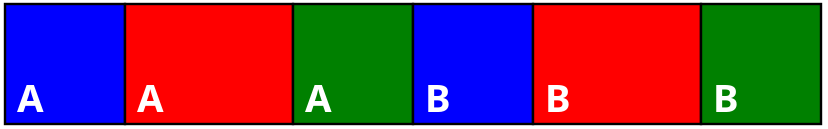
\includegraphics[width=\linewidth]{images/task_based_serial.png}
\caption{Task-based: una sola unità (esecuzione seriale).}
\label{fig:tb-1u}
\end{minipage}
\hfill
\begin{minipage}{0.48\textwidth}
\centering
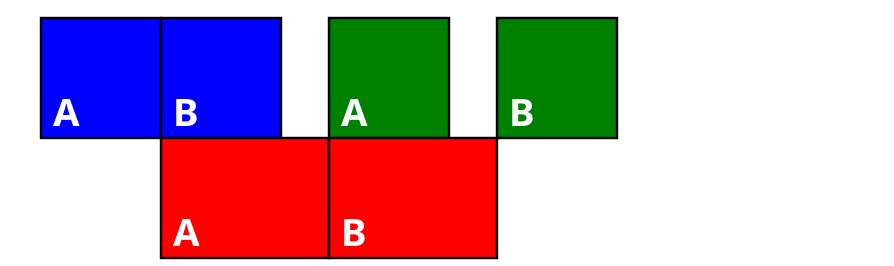
\includegraphics[width=\linewidth]{images/task_based_two_units_dependent.png}
\caption{Task-based: due unità, caso dipendente.}
\label{fig:tb-2u-dep}
\end{minipage}

\vspace{0.5cm}

\begin{minipage}{0.48\textwidth}
\centering
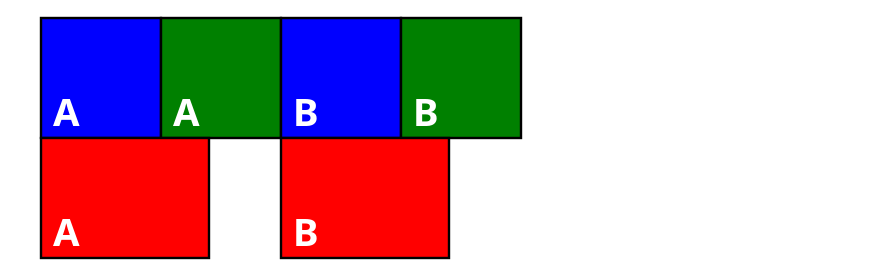
\includegraphics[width=\linewidth]{images/task_based_two_units_independent.png}
\caption{Task-based: due unità, caso indipendente.}
\label{fig:tb-2u-ind}
\end{minipage}
\hfill
\begin{minipage}{0.48\textwidth}
\centering
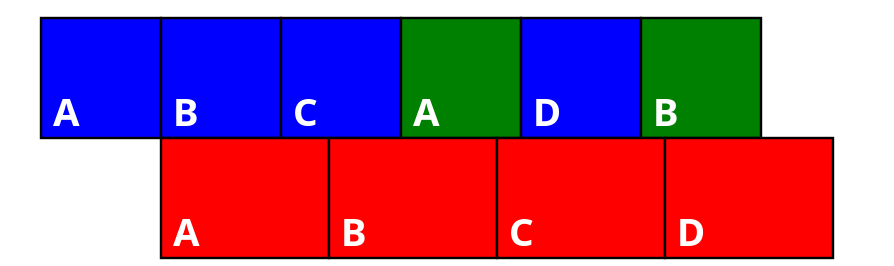
\includegraphics[width=\linewidth]{images/task_based_two_units_more_work_dependent.png}
\caption{Task-based: due unità, più lavoro, caso dipendente.}
\label{fig:tb-2u-dep-more}
\end{minipage}

\vspace{0.5cm}

\begin{minipage}{0.48\textwidth}
\centering
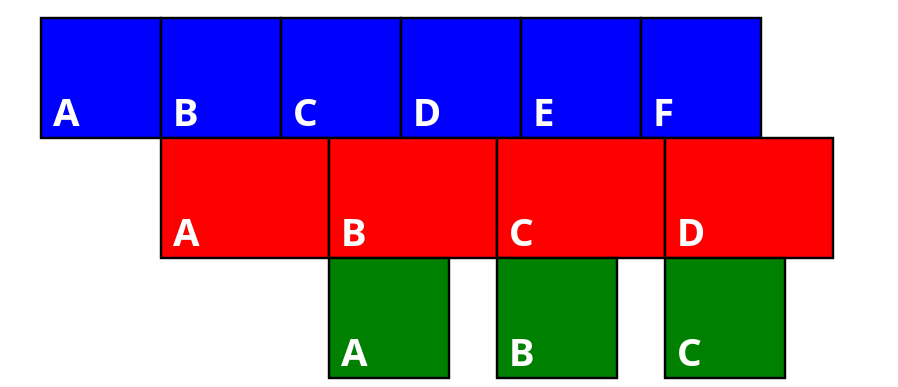
\includegraphics[width=\linewidth]{images/task_based_three_units_more_work_dependent.png}
\caption{Task-based: tre unità, più lavoro, caso dipendente.}
\label{fig:tb-3u-dep}
\end{minipage}
\hfill
\begin{minipage}{0.48\textwidth}
\centering
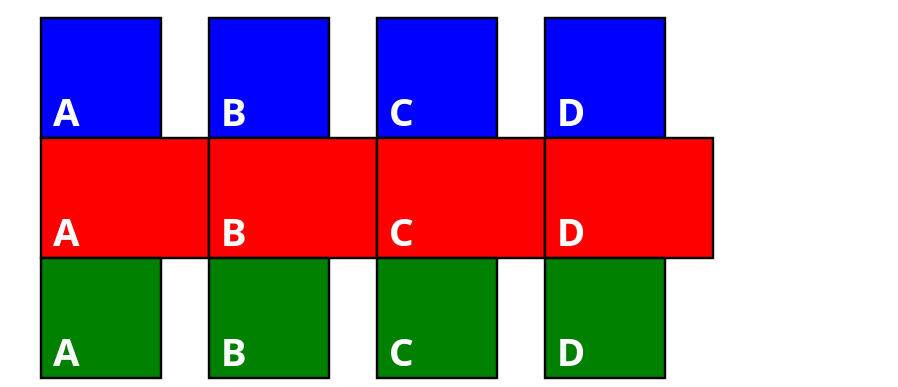
\includegraphics[width=\linewidth]{images/task_based_three_units_more_work_independent.png}
\caption{Task-based: tre unità, più lavoro, caso indipendente.}
\label{fig:tb-3u-ind}
\end{minipage}

\end{figure}

\subsection{Data-based parallelism}
Il data-based parallelism si basa sull'esecuzione di operazioni in parallelo su diversi dati. Tutte le unità computazionali fanno lo stesso lavoro, la divisione del lavoro avviene sui dati.  Si preferisce questo approccio quando:
\begin{itemize}
    \item Il lavoro può essere suddiviso in operazioni simili e semplici da eseguire su diversi dati.
    \item Si deve lavorare con una grossa mole di dati che può essere facilmente suddivisa in blocchi indipendenti.
\end{itemize}

\paragraph{Esempio: somma vettoriale.}

Un esempio classico di parallelismo \emph{data-based} è la somma vettoriale. 
Consideriamo due vettori $A$ e $B$ di lunghezza $N$ e un vettore risultato $C$, tale che:

\[
C_i = A_i + B_i \qquad i = 0, \dots, N-1
\]

In questo caso l'operazione da eseguire è la stessa per tutti gli elementi, mentre cambiano solo i dati su cui essa viene applicata. 
Questo rende il problema particolarmente adatto al parallelismo data-based, poiché ogni elemento del vettore può essere elaborato indipendentemente dagli altri.

\begin{description}
    \item[Seriale.] -  Nel caso \textbf{seriale} (Figura~\ref{fig:data-serial}) un'unica unità di calcolo esegue tutte le operazioni in sequenza. Per ogni indice $i$ vengono letti gli elementi $A_i$ e $B_i$, viene calcolata la somma e il risultato viene scritto nella posizione corrispondente del vettore $C$.  L'intero vettore viene quindi processato elemento per elemento.
    \item[Parallelo.] - Nel caso \textbf{parallelo} (Figura~\ref{fig:data-parallel}), invece, più unità di calcolo eseguono la stessa operazione contemporaneamente su elementi diversi dei vettori. 
    Ogni unità si occupa di un indice differente $i$, leggendo $A_i$ e $B_i$, calcolando la somma e scrivendo il risultato in $C_i$. 
    Poiché non esistono dipendenze tra le operazioni sui diversi elementi, tutte le somme possono essere eseguite in parallelo.  
\end{description}

\begin{figure}[h]
\centering

\begin{minipage}{0.48\textwidth}
\centering
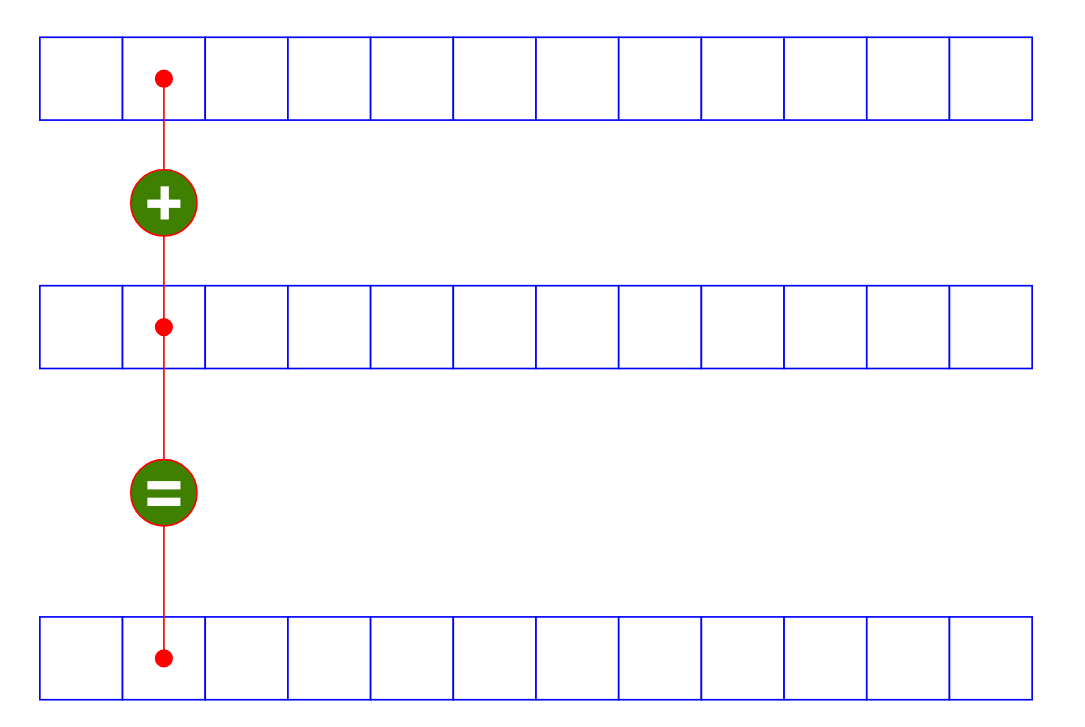
\includegraphics[width=\linewidth]{images/vector_add_serial.png}
\caption{Somma vettoriale eseguita in modo seriale.}
\label{fig:data-serial}
\end{minipage}
\hfill
\begin{minipage}{0.48\textwidth}
\centering
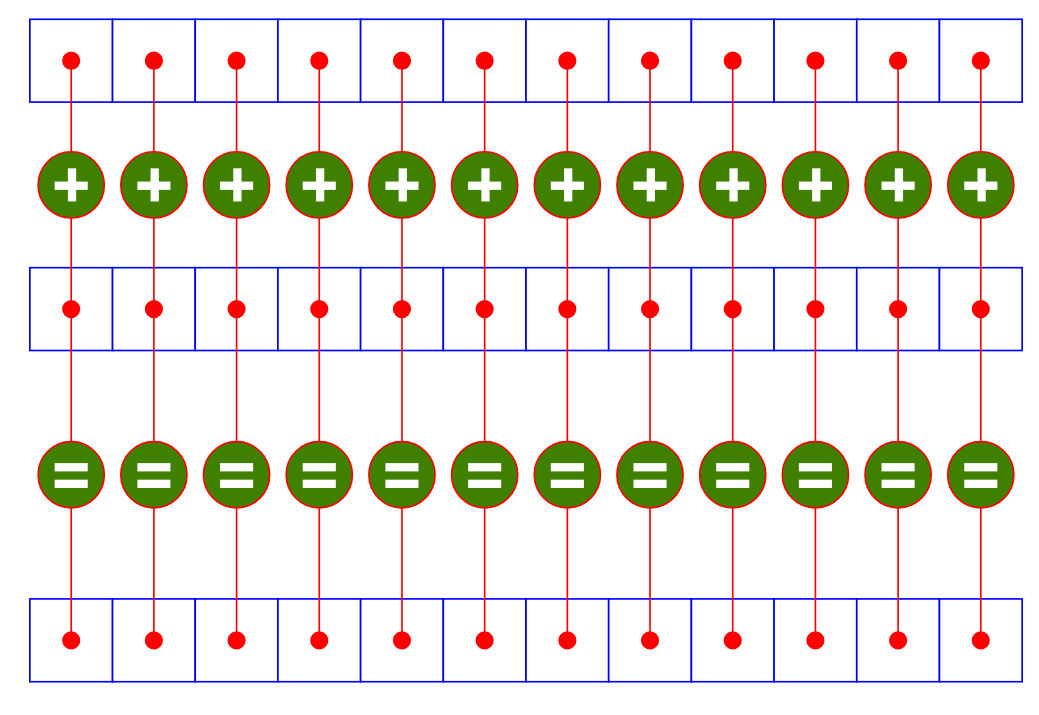
\includegraphics[width=\linewidth]{images/vector_add_parallel.png}
\caption{Somma vettoriale con parallelismo data-based.}
\label{fig:data-parallel}
\end{minipage}

\end{figure}

\section{Hardware per il calcolo parallelo}
L'hardware per il calcolo parallelo è progettato per supportare l'esecuzione simultanea di più operazioni. Si può classificare l'hardware parallelo in base a come gestisce le sue risorse di calcolo e, in particolare, di memoria.

\subsection{Shared memory}
In un'architettura a memoria condivisa, tutte le unità di calcolo accedono alla stessa memoria centrale. Questo permette una comunicazione semplice tra le unità, poiché possono leggere e scrivere direttamente sui dati condivisi. Questo modello ha una comunicazione più semplice e meno latenza, ma può essere limitato dalla contesa per l'accesso alla memoria e dalla scalabilità, poiché tutte le unità competono per le stesse risorse di memoria.

\subsection{Distributed memory}
In un'architettura a memoria distribuita, ogni unità di calcolo ha la propria memoria locale e non può accedere direttamente alla memoria delle altre unità. La comunicazione tra le unità avviene attraverso un sistema di messaggistica, in cui i dati devono essere esplicitamente inviati e ricevuti tra le unità. Questo modello è  più scalabile e non può essere soggetto a problemi di concorrenza, ma la comunicazione tra le unità è più complessa e può introdurre latenza significativa, soprattutto se i dati devono essere scambiati frequentemente.
 
\begin{figure}[htbp]
    \centering
    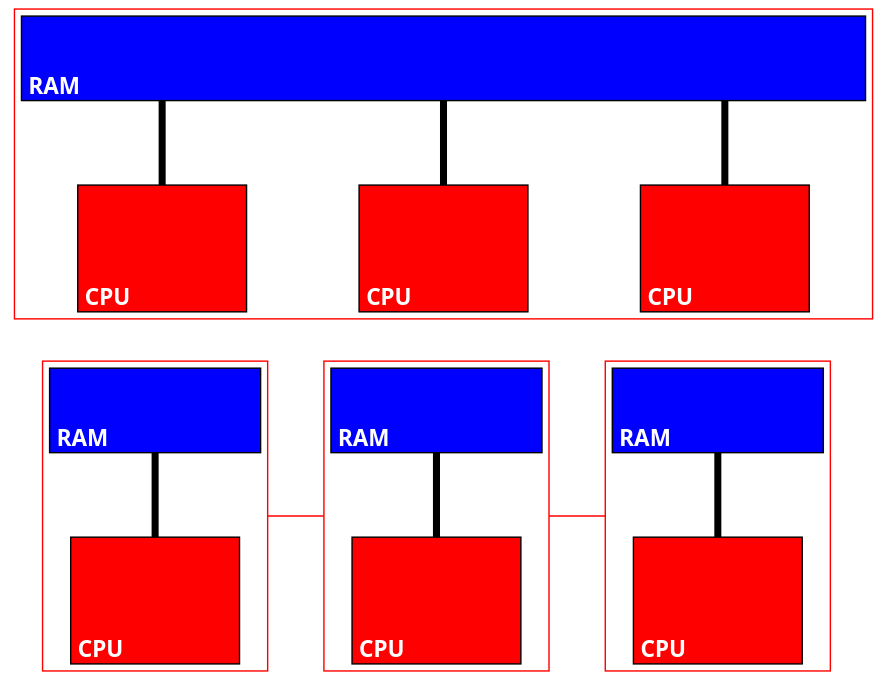
\includegraphics[width=0.8\textwidth]{images/shared_vs_distributed.png}
    \caption{Confronto tra architettura a memoria condivisa (in alto), dove più CPU accedono alla stessa RAM, e architettura a memoria distribuita (in basso), dove ogni nodo possiede memoria locale e comunica con gli altri.}
    \label{fig:shared-vs-distributed}
\end{figure}

\subsection{Ibrida}
Un'architettura ibrida combina elementi di entrambe le architetture a memoria condivisa e distribuita. In questo modello, le unità di calcolo sono organizzate in gruppi, dove ogni gruppo condivide una memoria locale, ma i gruppi stessi comunicano tra loro attraverso un sistema di messaggistica. Questo approccio cerca di bilanciare i vantaggi di entrambi i modelli, offrendo una maggiore scalabilità rispetto alla memoria condivisa, pur mantenendo una comunicazione più efficiente all'interno dei gruppi.

Un esempio sono i cluster di computer, dove ogni nodo del cluster ha la propria memoria locale, ma i nodi comunicano tra loro attraverso una rete ad alta velocità. All'interno di ogni nodo, le CPU possono accedere alla memoria condivisa, mentre tra i nodi la comunicazione avviene tramite messaggi.

\section{Concorrenza, latenza e banda}
Esistono misure di prestazioni per i sistemi paralleli che aiutano a comprendere l'efficienza e le limitazioni di un'architettura o di un algoritmo parallelo. Le principali sono:
\begin{description}
    \item[Latenza: ] la latenza è il tempo necessario per completare un'operazione, ovvero quello che intercorre tra la richiesta e la ricezione di un dato. In un sistema parallelo, la latenza può essere influenzata da fattori come la contesa per le risorse, la comunicazione tra unità di calcolo e la sincronizzazione tra processi. Una bassa latenza è desiderabile per garantire che le operazioni vengano completate rapidamente e che le unità di calcolo non restino inattive in attesa di completare le operazioni. La soluzione principale per minimizzare la latenza è limitare il numero di spostamenti di dati tra le varie unità.
    \item[Banda: ] la banda è la quantità di dati che può essere trasferita in un certo periodo di tempo. In un sistema parallelo, la banda è importante per garantire che i dati possano essere scambiati rapidamente tra le unità di calcolo, soprattutto in architetture a memoria distribuita. Una banda elevata è necessaria per evitare colli di bottiglia nella comunicazione e per garantire che le unità di calcolo possano accedere ai dati di cui hanno bisogno senza ritardi significativi.
    \item[Concorrenza: ] la concorrenza si riferisce alla capacità di un sistema di eseguire più operazioni contemporaneamente. In un sistema parallelo, la concorrenza è essenziale per sfruttare a pieno le risorse di calcolo disponibili. Tuttavia, la concorrenza può introdurre complessità nella gestione delle risorse, nella sincronizzazione tra processi e nella risoluzione di conflitti, soprattutto quando più processi accedono a dati condivisi. Per gestire la concorrenza in modo efficace esistono due soluzioni principali:
    \begin{itemize}
        \item Operazioni atomiche, ovvero operazioni che vengono eseguite in modo indivisibile, garantendo che nessun altro processo possa interferire durante la loro esecuzione.
        \item Semafori e/o mutex, che sono meccanismi di sincronizzazione che consentono di controllare l'accesso a risorse condivise, evitando conflitti e garantendo la coerenza dei dati.
    \end{itemize}
\end{description}

\paragraph{Esempio: latenza vs banda.}
Ipotizziamo una connessione ad alta velocità, come \emph{HyperTransport}, con il trasporto fisico di dati tramite un camion pieno di schede di memoria. 
Nel primo caso la bandwidth è di circa $50\ \text{GB/s}$ con una latenza massima di circa $256\ \text{ns}$. 
Nel secondo caso, considerando un camion carico di schede microSD, la quantità totale di dati trasportabili può essere estremamente elevata, raggiungendo una bandwidth teorica superiore a $1000\ \text{TB/s}$. 
Tuttavia, il tempo necessario affinché i dati arrivino a destinazione è dell'ordine delle ore, risultando quindi in una latenza molto elevata.

Per migliorare le prestazioni dei sistemi paralleli è quindi importante adottare alcune strategie:

\begin{itemize}
\item evitare trasferimenti inutili, in modo da utilizzare la bandwidth in maniera più efficiente;
\item accorpare più trasferimenti in operazioni più grandi, così da ammortizzare il costo della latenza.
\end{itemize}

\section{Richiesta e offerta di calcolo parallelo}
Il calcolo parallelo è diventato sempre più importante negli ultimi anni, sia per la crescente domanda di potenza di calcolo da parte di applicazioni complesse, sia per l'evoluzione dell'hardware che ha reso possibile l'esecuzione di operazioni in parallelo. 

\subsection{Domanda di calcolo parallelo}
Generalmente in contesti \textbf{scientifici}, \textbf{industriali} e \textbf{commerciali} si richiede un'elevata potenza di calcolo per affrontare problemi complessi, analizzare grandi quantità di dati e sviluppare applicazioni avanzate. Gli usi principali sono:
\begin{itemize}
    \item Monitoraggio: il calcolo parallelo consente di analizzare in tempo reale grandi quantità di dati provenienti da sensori, dispositivi IoT e sistemi di monitoraggio, permettendo di rilevare anomalie, prevedere guasti e ottimizzare le prestazioni.
    \item Simulazione: il calcolo parallelo è essenziale per eseguire simulazioni complesse in campi come la fisica, la chimica, l'ingegneria e la biologia, dove è necessario modellare fenomeni naturali, processi industriali o sistemi complessi.
    \item Analisi dei dati: il calcolo parallelo è fondamentale per l'analisi di grandi dataset, come quelli generati da social media, e-commerce, finanza e ricerca scientifica, consentendo di estrarre informazioni utili, identificare tendenze e prendere decisioni informate.
\end{itemize}

\subsection{Offerta di calcolo parallelo}
D'altra parte, l'offerta di calcolo parallelo è cresciuta significativamente grazie all'evoluzione dell'hardware e alla diffusione di tecnologie come i processori multi-core, le GPU e i cluster di computer. Queste tecnologie hanno reso possibile l'esecuzione di operazioni in parallelo su larga scala, offrendo una vasta potenza di calcolo. Oggi è possibile acquistare diverse soluzioni hardware per il calcolo parallelo, ciascuna con caratteristiche, vantaggi e limiti differenti.

\begin{description}

\item[Cluster:] rappresentano la soluzione più tradizionale su cui si è sviluppato il \emph{distributed computing}. 
Un cluster è composto da $n$ nodi, ciascuno dotato di CPU multi-core e memoria locale, collegati tra loro tramite una rete ad alta velocità. 
Questa architettura è ampiamente utilizzata in ambito scientifico e industriale per applicazioni che richiedono elevate capacità di calcolo.

I cluster costituiscono una soluzione classica e consolidata nel tempo, supportata da un vasto ecosistema software e da una grande diffusione di competenze tecniche. 
Offrono inoltre un'elevata flessibilità, poiché è possibile adattare l'infrastruttura a diverse tipologie di applicazioni.

D'altra parte, presentano anche alcuni svantaggi significativi. 
L'investimento iniziale in termini di hardware può essere molto elevato e i costi di manutenzione risultano spesso importanti, soprattutto per quanto riguarda il consumo energetico e i sistemi di raffreddamento. 
Inoltre il rapporto costo/prestazioni può risultare relativamente alto e l'efficienza energetica, misurata come prestazioni per watt consumato, non è sempre ottimale.

\item[GPU:] le unità di elaborazione grafica sono nate originariamente per l'elaborazione grafica nei videogiochi, ma nel tempo si è scoperto che la loro architettura altamente parallela poteva essere sfruttata anche per il calcolo generale. 
Da questa intuizione è nato il paradigma \emph{GPGPU} (\emph{General-Purpose computing on GPU}), che consente di utilizzare le GPU per eseguire calcoli scientifici e applicazioni ad alte prestazioni.

Le GPU offrono diversi vantaggi: il costo iniziale dell'hardware è generalmente inferiore rispetto a soluzioni basate su grandi cluster, così come i costi di manutenzione. 
Inoltre presentano un rapporto prezzo/prestazioni molto favorevole e un'elevata efficienza energetica, rendendole particolarmente adatte per applicazioni come machine learning, simulazioni numeriche e analisi di grandi quantità di dati.

Tuttavia, si tratta di una tecnologia relativamente più recente rispetto ai cluster tradizionali. 
Il modello di programmazione GPGPU ha iniziato a diffondersi solo a partire dalla fine del 2006 e dall'inizio del 2007, e per questo motivo l'ecosistema software è storicamente meno maturo. 
In alcuni contesti sono ancora disponibili meno strumenti, meno applicazioni consolidate e una minore diffusione di competenze specifiche, oltre a una flessibilità talvolta inferiore rispetto alle architetture più tradizionali.

\item[Acceleratori:] dispositivi specializzati che affiancano la CPU per eseguire operazioni specifiche in modo altamente parallelo. 
Questi componenti vengono utilizzati per migliorare le prestazioni in determinati ambiti applicativi, come l'elaborazione di segnali, la crittografia, il machine learning o il calcolo scientifico ad alte prestazioni. 
Gli acceleratori permettono di delegare alcune operazioni particolarmente intensive a hardware dedicato, aumentando l'efficienza complessiva del sistema.

\end{description}

\subsection{Videogiochi e GPU}
I videogiochi rappresentano un esempio di applicazione che richiede un'elevata potenza di calcolo parallelo, soprattutto per quanto riguarda l'elaborazione grafica. Le GPU sono state sviluppate proprio per soddisfare questa esigenza, consentendo di renderizzare scene complesse in tempo reale. I giochi moderni devono supportare:
\begin{itemize}
    \item Gameplay più sofisticato
    \item Grafiche più complesse
    \item Tre dimensioni
    \item Fisica più realistica
\end{itemize}
e per farlo devono sfruttare software e hardware migliori.

\paragraph{Esempio: software migliore.}
Un esempio storico di ottimizzazione software molto noto nel contesto dei videogiochi è l'algoritmo per il calcolo rapido dell'inversa della radice quadrata, utilizzato per velocizzare operazioni molto frequenti nella grafica 3D, come la normalizzazione dei vettori.

\begin{code}[caption={Implementazione approssimata della radice quadrata inversa},label={lst:rsqrt}]
float rsqrt(float x)
{
    float h = x/2;
    int i = *(int*)&x;
    i = 0x5f3758d - (i>>2);
    x = *(float*)&i;
    return x*(1.5f - h*x*x); /* newton */
}
\end{code}

Questo codice implementa una stima rapida di $1/\sqrt{x}$. 
L'idea è ottenere una prima approssimazione tramite una manipolazione diretta della rappresentazione binaria del numero floating-point e poi migliorarla con un'iterazione del metodo di Newton. L'efficienza di questo approccio deriva dal fatto che evita il calcolo diretto della radice quadrata, che storicamente era molto più costoso dal punto di vista computazionale. 

\paragraph{Esempio: hardware migliore.}
Per ottenere hardware migliore si possono seguire diverse strategie:
\begin{itemize}
    \item CPU più veloci, con frequenze di clock più elevate e architetture più efficienti. Questo ha un costo elevato e limita la scalabilità, poiché esistono limiti fisici alla velocità di clock e all'efficienza energetica delle CPU.
    \item Più dischi rigidi, per aumentare la capacità di archiviazione e migliorare le prestazioni di I/O. Tuttavia, questo approccio non migliora direttamente la potenza di calcolo e può introdurre colli di bottiglia nella gestione dei dati.
    \item Più memoria RAM e cache, per ridurre i tempi di accesso ai dati e migliorare le prestazioni complessive del sistema. Anche questo approccio ha limiti in termini di costo e scalabilità, poiché la memoria è una risorsa costosa e l'efficienza energetica può diminuire con l'aumentare della quantità di memoria.
    \item Hardware video dedicato, come le GPU, che offrono un'architettura altamente parallela e sono progettate per gestire carichi di lavoro specifici come l'elaborazione grafica. Questo approccio è particolarmente efficace per migliorare le prestazioni nei videogiochi, ma può essere meno flessibile rispetto a soluzioni più generiche come i cluster di CPU.
\end{itemize}

\section{Storia delle GPU}

\subsection{Dai primi adattatori video alle prime schede programmabili}

L'evoluzione delle GPU può essere interpretata come un progressivo aumento di quattro aspetti fondamentali: \textbf{risoluzione}, \textbf{numero di colori}, \textbf{accelerazione hardware} e \textbf{programmabilità}. Le prime schede video erano semplici adattatori grafici: \textbf{CGA} (1981) supportava $640\times 200$ in monocromatico oppure $320\times 200$ con 4 colori, oltre a modalità testuali con 16 colori. Con \textbf{EGA} (1984) si passa a $640\times 350$ con una palette di 16 colori scelta da un insieme di 64, ottenendo quindi una migliore qualità visiva sia in termini di dettaglio sia di rappresentazione cromatica.

Un salto più importante si ha con \textbf{VGA} (1987), che introduce 6 bit per colore per pixel, fino a 262\,144 colori rappresentabili, e modalità standard come $640\times 480$ con 16 colori da una palette di 256 e $320\times 200$ con 256 colori. VGA viene anche considerato il primo adattatore video pienamente programmabile. Nello stesso periodo compaiono soluzioni come \textbf{IBM 8514}, che oltre a supportare $1024\times 768$ con 256 colori in modalità interlacciata introducono l'accelerazione hardware di primitive 2D, come il disegno di linee, il riempimento di aree e il \emph{bit blit}. Con \textbf{XGA} (1990) si consolidano ulteriormente questi miglioramenti, con modalità come $800\times 600$ a 16 bit di colore e $1024\times 768$ con palette a 256 colori.

\subsection{La transizione verso la grafica 3D}

Negli anni Novanta, la diffusione delle interfacce grafiche e soprattutto dei videogiochi 3D cambia il ruolo delle schede video: non devono più soltanto visualizzare immagini, ma accelerare trasformazioni geometriche, illuminazione e rendering di scene tridimensionali. Nascono così le prime schede dedicate al 3D, che ottengono grande successo commerciale grazie a una grafica più pulita e animazioni più fluide.

Per rendere l'accesso a questo hardware più uniforme si affermano API standard come \textbf{OpenGL} e \textbf{DirectX}. Con l'introduzione del \textbf{programmable shading}, le schede video smettono di essere pipeline fisse e diventano dispositivi progressivamente programmabili: è in questo contesto che si diffonde il termine \textbf{GPU}.

\subsection{Dalla GPU al GPGPU}

Da qui nasce anche l'idea di utilizzare la GPU non solo per la grafica ma anche per il calcolo generale. In una prima fase, intorno al 2004, i problemi numerici venivano trasformati artificialmente in problemi grafici e risolti tramite il rendering, in modo complesso ma spesso efficace. La vera svolta arriva quando i produttori rendono accessibile in modo diretto la potenza di calcolo delle GPU: \textbf{ATI/AMD} con \textbf{CAL} e \textbf{NVIDIA} con \textbf{CUDA}. Da questo momento la GPU non è più soltanto un acceleratore grafico, ma una vera piattaforma di calcolo parallelo programmabile.

\section{GPU moderne}
Oggi le GPU sono dispositivi estremamente potenti e versatili, utilizzati non solo per la grafica ma anche per una vasta gamma di applicazioni scientifiche, industriali e commerciali. Le GPU moderne sono caratterizzate da un'architettura altamente parallela, si parla di centinaia di multi-processori ognuno equipaggiato con circa 100 \textbf{Processing Unit} (come i CUDA core di NVIDIA), che consentono di eseguire migliaia di thread contemporaneamente. Una processing unit è un'unità di calcolo che esegue operazioni aritmetiche e logiche sui dati, ed è progettata per gestire carichi di lavoro altamente paralleli.

\subsection{GPU e CPU: performance e costi}
Le GPU e le CPU sono progettate per scopi diversi e presentano caratteristiche architetturali differenti, che is riflettono molto sulle prestazioni finali. Le GPU sono ottimizzate per eseguire un gran numero di operazioni in parallelo, con un'architettura che consente di gestire migliaia di thread contemporaneamente. Le CPU, invece, sono progettate per eseguire operazioni più complesse e meno parallelizzabili, con un numero limitato di core e una maggiore enfasi sulla latenza. Inoltre, mentre le GPU sono indicate per il parallelismo \emph{task-based}, le CPU sono indicate per il parallelismo \emph{data-based}.

Dalle tabelle riportate in Tabella~\ref{tab:gpu_cpu_performance} si può notare che le GPU offrono un numero significativamente maggiore di unità di elaborazione (MPs) e una maggiore potenza di calcolo in termini di FLOPS rispetto alle CPU.
Inoltre, le GPU tendono ad avere una banda di memoria molto più elevata rispetto alle CPU, il che è cruciale per gestire i grandi volumi di dati necessari per le applicazioni di calcolo parallelo. Tuttavia, è importante considerare anche i costi associati all'acquisto e alla manutenzione di questi dispositivi, nonché la complessità dell'ecosistema software e la disponibilità di competenze specifiche per sfruttare a pieno le potenzialità delle GPU. 

\begin{table}[h]
\centering
\begin{tabular}{lcccc}
\multicolumn{5}{c}{\textbf{GPU vs CPU: performance}} \\[0.3em]
\hline
\textbf{Model} & \textbf{MPs} & \textbf{PE/MP} & \textbf{FLOPS (TFLOPS)} & \textbf{bandwidth (GB/s)} \\
\hline
AMD Radeon VII   & 60 & 64 & 11.1 & 1028 \\
NVIDIA TITAN RTX & 72 & 64 & 12.4 & 672 \\
\hline
\end{tabular}

\vspace{0.8cm}

\begin{tabular}{lcccc}
\textbf{Model} & \textbf{cores} & \textbf{PE/core} & \textbf{FLOPS (GFLOPS)} & \textbf{bandwidth (GB/s)} \\
\hline
AMD EPYC 7702P 2GHz      & 64 & 16 & 4096 & 143.1 \\
Intel Xeon W-3275M 2.5GHz & 28 & 32 & 3072 & 131.13 \\
\hline
\end{tabular}
\caption{Confronto prestazionale tra alcune GPU e CPU.}
\label{tab:gpu_cpu_performance}
\end{table}

\paragraph{APU.}
Una terza opzione è rappresentata dalle APU (\textbf{Accelerated Processing Unit}), che integrano CPU e GPU su un unico chip. Le APU offrono un compromesso tra le prestazioni di calcolo parallelo delle GPU e la flessibilità delle CPU, consentendo di eseguire sia operazioni generali che specifiche per la grafica in modo efficiente. Tuttavia, le APU tendono ad avere prestazioni inferiori rispetto a soluzioni dedicate come le GPU discrete, ma possono essere una scelta interessante per applicazioni che richiedono un equilibrio tra potenza di calcolo e costi.

\section{Parallelizzazione}

\subsection{Concetto generale di parallelizzazione}

La parallelizzazione è il processo di suddivisione di un problema o di un algoritmo seriale in un algoritmo parallelo. Ipotizziamo due estremi:
\begin{description}
    \item[Un algoritmo intrinsecamente seriale] è un algoritmo che non può essere parallelizzato, poiché vi è una dipendenza tra le operazioni che rende impossibile eseguirle in contemporanea (ad esempio, un'operazione dipende dai risultati delle operazioni precedenti). In questo caso, l'unico modo per eseguire l'algoritmo è in modalità sequenziale, e lo speed-up ottenibile con il calcolo parallelo è limitato. Tuttavia un modo per parallelizzare un algoritmo seriale è quello di fare parallelismo \emph{data-based}, ovvero eseguire in parallelo operazioni simili su dati diversi, anche se l'algoritmo stesso non è parallelizzabile.
    \item[Un algoritmo intrinsecamente parallelo] è un algoritmo che può essere suddiviso in parti indipendenti che possono essere eseguite contemporaneamente. In questo caso, è possibile ottenere uno speed-up significativo utilizzando più unità di calcolo, poiché le operazioni possono essere eseguite in parallelo senza dipendenze.
\end{description}

\subsection{Algoritmi apparentemente seriali}

Esistono però vie di mezzo, ovvero algoritmi che non sono intrinsecamente seriali ma che possono essere parallelizzati se interpretati in maniera differente. Alcuni esempio sono:
\begin{itemize}
    \item Riduzione: operazioni che combinano più elementi in un unico risultato, come la somma di un array o il prodotto di matrici. Questi algoritmi possono essere parallelizzati suddividendo i dati in blocchi e combinando i risultati parziali. Tuttavia, la parallelizzazione ha un requisito: è necessario (e sufficiente) che l’operazione sia associativa.
    \item Scan: operazioni che producono un array di risultati parziali, come la somma cumulativa o il prefisso di un array. Questi algoritmi possono essere parallelizzati utilizzando tecniche come il \emph{divide and conquer} per suddividere i dati e combinare i risultati.
    \item Algoritmi di ordinamento: algoritmi come il merge sort o il quicksort possono essere parallelizzati suddividendo l'array in parti più piccole e ordinando ciascuna parte in parallelo, per poi combinare i risultati.
\end{itemize}

\subsection{Parallelismo in hardware}

Dal punto di vista dell'hardware, esistono diversi modelli con cui il parallelismo può essere implementato. I principali sono:

\begin{description}
    \item[SIMD] (\emph{Single Instruction, Multiple Data}) indica un modello in cui una singola istruzione opera contemporaneamente su più dati. Questo approccio è tipico delle istruzioni vettoriali presenti nelle CPU moderne, come MMX, AltiVec, SSE, NEON o AVX, ed è particolarmente efficace quando si devono eseguire gli stessi calcoli su vettori o array.
    
    \item[SPMD] (\emph{Single Program, Multiple Data}) indica un modello nel quale la stessa sequenza di istruzioni viene eseguita da più unità di calcolo contemporaneamente su dati differenti. In questo caso non si parla necessariamente di una singola istruzione eseguita nello stesso istante, ma dello stesso programma applicato a porzioni diverse dell'input. Questo modello può essere supportato sia dall'hardware sia dal software.
    
    \item[SIMT] (\emph{Single Instruction, Multiple Threads}) è un modello tipico delle GPU. In questo caso l'hardware gestisce automaticamente gruppi di thread che eseguono la stessa istruzione in parallelo. Si tratta quindi di un modello vicino a SPMD, ma con una gestione dei thread fortemente integrata a livello hardware.
\end{description}

In generale, si può osservare che le \textbf{GPU} moderne sono tipicamente associate ai modelli \textbf{SPMD} e \textbf{SIMT}, mentre le \textbf{CPU} moderne sono principalmente \textbf{SIMD}, eventualmente affiancate da forme di SPMD controllate dal software.

\subsection{Parallelismo in software}

Dal punto di vista software, il parallelismo può essere organizzato secondo modelli differenti. I principali sono:

\begin{description}
    \item[Multi-processing] è il parallelismo basato su più thread in memoria condivisa. In questo caso un singolo programma genera più thread che operano sullo stesso spazio di memoria condiviso. Questo modello è tipico dei sistemi multicore e lo standard più diffuso su CPU è \textbf{OpenMP}.
    
    \item[Message-passing] è un modello nel quale più processi distinti comunicano tra loro scambiandosi messaggi. Questo approccio è naturale nei sistemi a memoria distribuita, dove ogni processo possiede una propria memoria locale e la cooperazione avviene tramite comunicazione esplicita. Lo standard di riferimento in questo ambito è \textbf{MPI} (\emph{Message Passing Interface}).
    
    \item[Hybrid] combina i due modelli precedenti: più processi comunicano tramite messaggi e, all'interno di ciascun processo, sono presenti più thread. Questo modello è molto comune nei sistemi HPC moderni, poiché consente di sfruttare contemporaneamente il parallelismo interno ai nodi e quello tra nodi diversi.
\end{description}